\documentclass[11pt]{article}

% Paquetes
%===================================================================================================

% Establecemos los márgenes
\usepackage[a4paper, margin=1in]{geometry}

% Separacion entre parrafos
\setlength{\parskip}{1em}

% Paquete para incluir codigo
\usepackage{listings}

% Paquete para incluir imagenes
\usepackage{graphicx}
\graphicspath{ {./imagenes/} }

% Para fijar las imagenes en la posicion deseada
\usepackage{float}

% Para que el codigo acepte caracteres en utf8
\lstset{literate=
  {á}{{\'a}}1 {é}{{\'e}}1 {í}{{\'i}}1 {ó}{{\'o}}1 {ú}{{\'u}}1
  {Á}{{\'A}}1 {É}{{\'E}}1 {Í}{{\'I}}1 {Ó}{{\'O}}1 {Ú}{{\'U}}1
  {à}{{\`a}}1 {è}{{\`e}}1 {ì}{{\`i}}1 {ò}{{\`o}}1 {ù}{{\`u}}1
  {À}{{\`A}}1 {È}{{\'E}}1 {Ì}{{\`I}}1 {Ò}{{\`O}}1 {Ù}{{\`U}}1
  {ä}{{\"a}}1 {ë}{{\"e}}1 {ï}{{\"i}}1 {ö}{{\"o}}1 {ü}{{\"u}}1
  {Ä}{{\"A}}1 {Ë}{{\"E}}1 {Ï}{{\"I}}1 {Ö}{{\"O}}1 {Ü}{{\"U}}1
  {â}{{\^a}}1 {ê}{{\^e}}1 {î}{{\^i}}1 {ô}{{\^o}}1 {û}{{\^u}}1
  {Â}{{\^A}}1 {Ê}{{\^E}}1 {Î}{{\^I}}1 {Ô}{{\^O}}1 {Û}{{\^U}}1
  {ã}{{\~a}}1 {ẽ}{{\~e}}1 {ĩ}{{\~i}}1 {õ}{{\~o}}1 {ũ}{{\~u}}1
  {Ã}{{\~A}}1 {Ẽ}{{\~E}}1 {Ĩ}{{\~I}}1 {Õ}{{\~O}}1 {Ũ}{{\~U}}1
  {œ}{{\oe}}1 {Œ}{{\OE}}1 {æ}{{\ae}}1 {Æ}{{\AE}}1 {ß}{{\ss}}1
  {ű}{{\H{u}}}1 {Ű}{{\H{U}}}1 {ő}{{\H{o}}}1 {Ő}{{\H{O}}}1
  {ç}{{\c c}}1 {Ç}{{\c C}}1 {ø}{{\o}}1 {å}{{\r a}}1 {Å}{{\r A}}1
  {€}{{\euro}}1 {£}{{\pounds}}1 {«}{{\guillemotleft}}1
  {»}{{\guillemotright}}1 {ñ}{{\~n}}1 {Ñ}{{\~N}}1 {¿}{{?`}}1 {¡}{{!`}}1
}

% Para que no se salgan las lineas de codigo
% Para fijar una fuente que resalte
\lstset{breaklines=true, basicstyle=\ttfamily}

% Para que los metadatos que escribe latex esten en español
\usepackage[spanish]{babel}
\decimalpoint % Para que no se cambie el punto a la coma

% Para la bibliografia
% Sin esto, los enlaces de la bibliografia dan un error de compilacion
\usepackage{url}

% Para que se puedan clicar los enlaces
\usepackage{hyperref}

% Para mostrar graficas de dos imagenes, cada una con su caption, y con un caption comun
\usepackage{subcaption}

% Simbolo de los numeros reales
\usepackage{amssymb}

% Para que los codigos tengan una fuente distinta
\usepackage{courier}

\lstdefinestyle{CustomStyle}{
  language=Python,
  numbers=left,
  stepnumber=1,
  numbersep=10pt,
  tabsize=4,
  showspaces=false,
  showstringspaces=false
  basicstyle=\tiny\ttfamily,
}

% Para referenciar secciones usando el nombre de las secciones
\usepackage{nameref}

% Para enumerados dentro de enumerados
\usepackage{enumitem}

% Para mejores tablas
\usepackage{tabularx}

% Para poder tener el mismo identificador en dos tablas separadas
\usepackage{caption}

% Mostrar la página de las referencias en el indice del documento
\usepackage[nottoc,numbib]{tocbibind}

% Para mostrar las matrices
\usepackage{amsmath}

% Para que las notas al pie de pagina queden bien abajo
\usepackage[bottom]{footmisc}

% Comandos personalizados
%===================================================================================================

% Para realizar las citas de forma corta
\newcommand{\customcite}[1]{\emph{"\ref{#1}. \nameref{#1}"}}

% Para entrecomillar un texto
\newcommand{\entrecomillado}[1]{\emph{``#1''}}

% Metadatos del documento
%===================================================================================================
\title{
    {Inteligencia de Negocio - Práctica 2} \\
    {Análisis Relacional mediante Segmentación}
}

\author{
    {Sergio Quijano Rey - 72103503k}\\
    {sergioquijano@correo.ugr.es} \\
    {5º Doble Grado Ingeniería Informática y Matemáticas} \\
    {Grupo de prácticas 1}
}

\date{\today}

% Separacion entre parrafos
\setlength{\parskip}{1em}

% Contenido del documento
%===================================================================================================
\begin{document}

% Portada del documento
\maketitle
\pagebreak

% Indice de contenidos
\tableofcontents

% Lista de figuras
% Uso el addtocontents para que no se muestre la seccion de indice de figuras en el indice inicial

\addtocontents{toc}{\setcounter{tocdepth}{-10}}
\listoffigures

% TODO -- no tenemos cuadros en esta memoria
% \listoftables

% TODO -- tampoco tenemos codigos de relevancia
% \lstlistoflistings
\addtocontents{toc}{\setcounter{tocdepth}{3}}

\pagebreak

\section{Introducción}

\subsection{Problema a resolver}

En esta práctica, trabajaremos con un conjunto de datos del \entrecomillado{Instituto Nacional de Estadística}. En concreto, trabajamos con la \entrecomillado{Encuesta de condiciones de vida, 2020} \cite{original_dataset:online}. En términos del \entrecomillado{INE}, trabajamos con microdatos, lo que nos va a permitir realizar estudios en profundidad sobre la encuesta estudiada, más allá de los resúmenes basados en el estudio de las frecuencias, clásicos de las encuestas.

\subsection{Notas previas}

Todo el código de la práctica está documentado tanto con comentarios propios de \lstinline{Python} como con celdas de \lstinline{Markdown}. Además, organizamos el código en las mismas secciones que presentamos en esta memoria. Por tanto, hacemos referencia al nombre de las funciones cuando sea necesario, sin incluir trozos de código en la memoria.

\subsection{Resumen de la forma de proceder}

Aunque más adelante, en el desarrollo de cada caso de estudio, se haga claro el procedimiento considerado, lo resumimos aquí de forma previa.

En cada caso de estudio, empezaremos definiendo el filtro que fija el caso de estudio en sí. Esto es, definimos la condición que filtrará las filas de nuestro conjunto de datos que estudiamos. Además, definimos las variables que consideramos, es decir, definimos las columnas del \emph{dataset} que consideramos para este caso de estudio.

Realizamos un procesado básico de los datos (borrado de datos faltantes, datos \lstinline{NaN}, borrado de \emph{outliers} y normalización). A partir de este procesado, realizamos cierto análisis exploratorio de datos, para tomar ideas a la hora de atacar cada problema en concreto.

A continuación, aplicamos los algoritmos de \emph{clustering}, mostrando gráficamente el resultado obtenido. Una vez ejecutados todos los algoritmos, calculamos un conjunto de métricas sobre los etiquetados generados, para poder comparar los resultados de los algoritmos. Visualizamos estas métricas y proyecciones del etiquetado a un espacio bidimensional (usando \emph{PCA} y \emph{tsne}).

Seguidamente, exploramos los parámetros de un par de algoritmos por cada caso de estudio, en busca de encontrar unos parámetros optimales para realizar la \emph{clusterización}.

Para finalizar, en esta memoria realizamos unas conclusiones, tanto del comportamiento de los algoritmos empleados como del conocimiento extraído sobre el conjunto de datos, gracias a las técnicas que hemos empleado.

\subsection{Observaciones y secciones previas}

Todo el código lo hemos organizado en un único \emph{Notebook} de \emph{Jupyter}. Para mantener el orden, hemos agrupado el código en secciones y subsecciones. Se puede explorar cómodamente esta jerarquía empleando \emph{Jupyter Lab} en vez de \emph{Jupyter Notebook}, o directamente empleado \emph{Google Colab}.

Hemos desarrollado una \textbf{sección inicial} con funcionalidades que vamos a estar usando durante todo el \emph{notebook}, evitando así repetir excesivamente el mismo código. Además, con esto, en las secciones de los casos de estudio nos centramos más en plantear ideas y ver los resultados, evitando toda la suciedad que supondría colocar en medio de estos desarrollos todo el código con la implementación. Esta sección previa de código común se divide en las siguientes subsecciones:

\begin{enumerate}
    \item Un decorador de \lstinline{Python} para poder medir fácilmente, y sin complicar el código, las funciones que calculan los \emph{clusters}. Esto es básico pues es una métrica que debemos estudiar, y que las librerías que estamos usando (principalmente \lstinline{sklearn}), no nos aportan de forma fácil
    \item Funciones para calcular \emph{clusters}. Destaca la función \lstinline{add_clustering_labels}, que toma como parámetro una función de clusterización con sus parámetros, y se encarga de calcular la clusterización y añadir las etiquetas al \lstinline{dataframe} convenientemente. Además, podemos especificar qué columnas ignorar en el \lstinline{dataframe} a la hora de calcular la clusterización (para no usar columnas con etiquetas de otros algoritmos, principalmente)
    \item Funciones para evaluar \emph{clusters}. En esta subsección definimos unas cuantas métricas que usaremos para comparar los resultados. La función \lstinline{compute_clustering_metrics} agrupa todas estas métricas y las devuelve convenientemente en un diccionario de \lstinline{Python}.
    \item Funciones para realizar visualizaciones. Con esto es más fácil usar las funciones de \lstinline{seaborn}, evitando tener que repetir código para, por ejemplo, excluir ciertas columnas del \lstinline{dataframe}. Destaca la función \lstinline{plot_centroids_with_size}. En esta función:
    \begin{itemize}
        \item Calculamos con código propio, por cada \emph{cluster}, el centroide y el radio de este, y el número de elementos en cada \emph{cluster}
        \item Aplicamos \emph{tsne} como técnica de proyección en un espacio bidimensional de los datos de entrada
        \item Con esta proyección, mostramos gráficamente los centroides obtenidos en la \emph{clusterización}, con un tamaño proporcional al radio previamente calculado, y con un color proporcional al número de elementos de cada \emph{cluster}
    \end{itemize}
    \item Funciones para procesar los \emph{dataframes}. Con esto, evitamos repetir el código que normaliza los datos, borra datos \lstinline{NaN} y borra \emph{outliers}
\end{enumerate}

Antes de pasar a los casos de estudio, debemos comentar otras dos secciones, la sección de filtrado previo del \emph{dataset} global y la sección de variables añadidas.

En la \textbf{sección de filtrado previo del \emph{dataset} global}, definimos el conjunto de variables que nos interesan, descartando el resto por completo. Esta selección se realizó al principio del desarrollo de la práctica, buscando una primera exploración del conjunto de datos. Por esto se seleccionan variables que más tarde no se usan para nada. Pero decidimos dejar estas variables en el \emph{Notebook}  como ilustración de cuál fue nuestro proceso a la hora de abordar el problema. Nos quedamos, en esta fase, con un total de \textbf{39 variables}.

En la \textbf{sección de variables añadidas}, definimos algunas variables agregadas (que combinan información de varias variables, o que transforman la información en bruto) a nuestro \emph{dataset}. En concreto:

\begin{itemize}
    \item Definimos la variable \lstinline{booleana} \lstinline{pidio_ayuda} que controla si un hogar pidió o no pidió ayuda, ya sea a un familiar o a otro tipo de entidad.
    \item Definimos la variable \lstinline{gasto_transporte_total} que combina el gasto en transporte público y transporte privado
    \item Definimos la variable \lstinline{retraso_pago}, que controla si se produjo cualquier tipo de retraso en los pagos
    \item Definimos la variable \lstinline{ingresos_menos_gastos}, que realiza la resta de todos los ingresos de un hogar menos todos los gastos, registrados en el \emph{dataset}, de ese hogar
    \item Definimos la variable ordinal \lstinline{comunidad_autonoma_code}, que convierte el código en texto de una comunidad autónoma a una variable entera. Esto con la intención de poder usar esta variable en los algoritmos de \emph{clusterización}
    \item Definimos la variable \lstinline{habitaciones_por_persona} que calcula el cociente del número de integrantes de un hogar entre el número de habitaciones de dicho hogar
\end{itemize}

Con todo esto, pasamos a tener un total de \textbf{45 variables}. De nuevo, algunas de estas variables añadidas no se usan en los casos de estudio, pero las dejamos para ilustrar el proceso realizado en la búsqueda de casos de estudio interesantes.

A partir de este punto ya nos encontramos con las secciones propias a los casos de estudio, que pasamos a comentar en cada sección correspondiente.

\pagebreak

\section{Caso de estudio 1}

\subsection{Definición del caso de estudio}

En este caso de estudio queremos poner nuestra atención en aquellas personas que \textbf{viven en un entorno en el que hay vandalismo}. Para ello usamos la variable \lstinline{vandalismo_en_la_zona}, que se corresponde con el código \lstinline{"HS190"}.

Una vez filtradas las filas que vamos a estudiar, filtramos las variables (columnas) que nos interesan. En concreto, nos quedamos con la renta disponible del hogar, los gatos mensuales de la vivienda, el gasto total en transporte y los códigos de la comunidad autónoma. Nos interesa realizar los siguientes estudios:

\begin{itemize}
    \item Estudiar la distribución del vandalismo por cada comunidad autónoma
    \item Estudiar el uso del transporte en las zonas conflictivas
    \item Lógicamente, nos interesa el factor económico involucrado en definir zonas posiblemente conflictivas. La hipótesis básica es que en las zonas de menor renta hay más vandalismo. Pero también puede haber vandalismo en las zonas más pudientes (robos, asaltos a casas, \ldots)
    \item El gasto en vivienda puede ser interesante como otra variable para fijar el estatus socio-económico. En ciertas comunidades autónomas, un alto gasto en vivienda no significa un nivel alto de vida (precios demasiado inflados, precios en zonas urbanas mucho más altos que en zonas rurales, \ldots)
\end{itemize}

Además, en el \emph{dataframe} que usamos para almacenar estos datos (\lstinline{df_study_case}), guardamos el factor de elevación, que usaremos para ponderar los ejemplos, en aquellos algoritmos que acepten este parámetro de ponderación.

Tras el filtrado, obtenemos un \emph{dataset} con 2081 filas (objetos a \emph{clusterizar}) y 5 columnas (4 + 1 para el factor de elevación).

\pagebreak

\subsection{Procesado de los datos}

Como ya hemos comentado previamente, realizaremos el siguiente pre-procesado de los datos:

\begin{itemize}
    \item Borrado de las filas que contengan algún valor \lstinline{NaN}
    \item Borrado de \emph{outliers} usando la regla $3 \cdot IQR$, variable por variable
    \item Normalización del rango de las variables al intervalo $[0, 1]$
\end{itemize}

Tras aplicar esto, nos quedamos con un \emph{dataset} de 1947 filas.

\pagebreak

\subsection{Análisis Exploratorio de datos}

Comenzamos haciendo un \emph{plot} por pares de variables, que mostramos en la siguiente figura:

\begin{figure}[H]
    \centering

    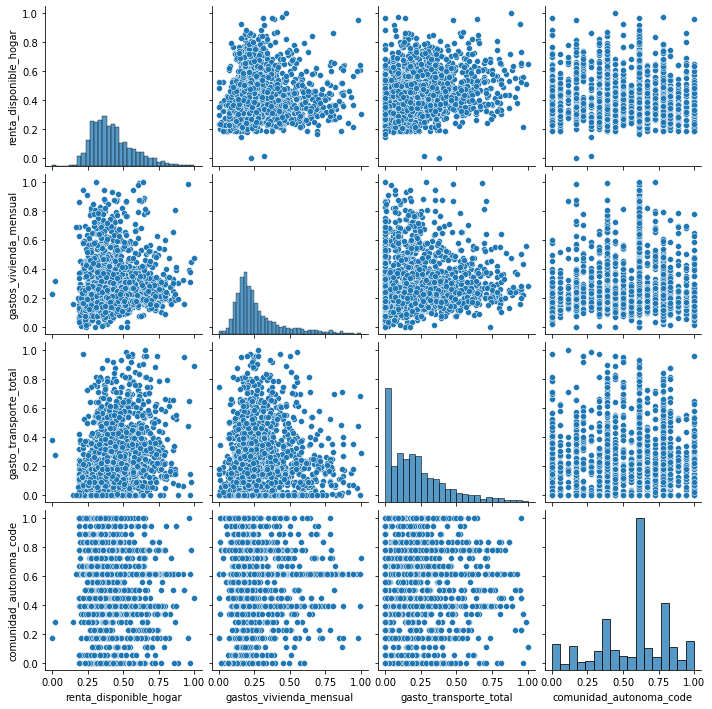
\includegraphics[width = 0.9 \textwidth]{stcase01_pairplot}
    \caption{Gráfico en el que se muestran todas las combinaciones de parejas de variables involucradas en el caso de estudio}
    \label{stcase01_pairplot:figura}
\end{figure}

En este gráfico tenemos las distribuciones al poner en un eje una variable y en el otro eje otra variable, considerando todas las parejas posibles. En la diagonal tenemos la distribución de cada variable, por sí sola.

Lo que más llama la atención de este gráfico es que, en la distribución de las comunidades autónomas, hay una comunidad que destaca claramente sobre otras. Esto podría ser porque dicha comunidad autónoma tiene una mayor representación en la encuesta, o no. Por tanto, es necesario visualizar dicha distribución de forma porcentual, considerando como base para el cálculo (el valor del denominador para el cálculo del porcentaje) toda la población encuestada de cada comunidad.

El resto de distribuciones tienen una forma parecida a la normal, lo que era de esperar. Salvo la distribución del gasto en transporte, donde el gasto mínimo (puede que no sea nulo, pues hemos normalizado las variables al rango $[0, 1]$) destaca sobre el resto de valores, rompiendo con una distribución normal que esperábamos.

Se puede apreciar cierta correlación positiva entre la renta disponible en el hogar y el gasto en vivienda mensual. Pero parece ser una correlación muy débil y que no destaca nada interesante (es lógico que a mayor dinero disponible, generalmente se gaste más en vivienda).

La correlación entre gasto en vivienda y gasto en transporte no parece aportar nada nuevo al estudio que queremos realizar.

Por la naturaleza ordinal del código de la comunidad autónoma, no podemos extraer mucha información al respecto usando esta gráfica y esta variable en concreto.

Como comentábamos previamente, destaca los picos de ciertas comunidades autónomas en el número de hogares que viven en un entorno de vandalismo. Pero esto puede deberse a diferencias en tamaños de las comunidades. Así que pasamos a mostrar el porcentaje de hogares que viven en entornos con vandalismo, agrupados por comunidades autónomas:

\begin{figure}[H]
    \centering

    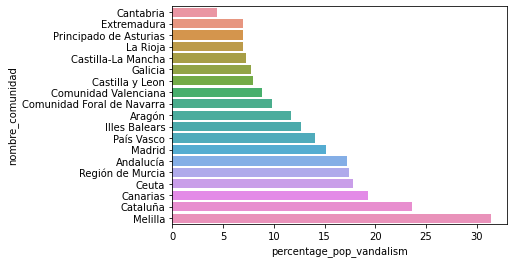
\includegraphics[width = 0.8 \textwidth]{stcase01_porcentajes_vandalismo}
    \caption{Gráfico con el porcentaje de hogares que viven en entornos con vandalismo, agrupados por comunidades autónomas}
\end{figure}

En este gráfico podemos ver que, como suponíamos, hay ciertas comunidades autónomas con un porcentaje de hogares en zonas con vandalismo mucho mayores que otras comunidades. Destaca la ciudad autónoma de Melilla, que se distancia de la segunda peor comunidad según esta métrica prácticamente un 10\%. Además, a la vista de estos datos, y sin necesidad de introducir datos externos sobre poblaciones de las comunidades autónomas, parece que las zonas más rurales y con menos concentración de población (Cantabria, Extremadura, Asturias, \ldots) tienen porcentajes de vandalismo significativamente menor que comunidades más densamente pobladas (Cataluña, Andalucía, Madrid, \ldots). Destacan, saliéndose de lo que acabamos de comentar, las dos ciudades autónomas.

A continuación, mostramos el gasto medio en transporte público según si se vive en una zona con vandalismo o no:

\begin{figure}[H]
    \centering

    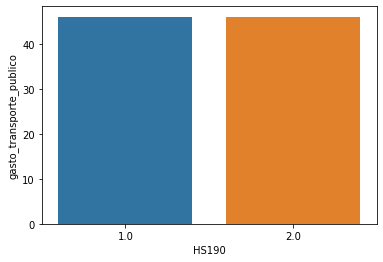
\includegraphics[width = 0.6 \textwidth]{stcase01_gasto_tpublico_vandalismo}
    \caption{Media de gasto en transporte público. A la izquierda, media de gasto en la población que vive en zonas con vandalismo. A la derecha, media de gasto en la población que vive en zonas sin vandalismo}
\end{figure}

A vista de estos resultados, no podemos sacar conclusiones de interés sobre un comportamiento distinto de las dos poblaciones. La media es prácticamente la misma. Como la media no está siendo lo suficientemente informativa (estamos resumiendo demasiado toda la información de las poblaciones), mostramos las distribuciones de gasto en transporte público en las dos poblaciones:


\begin{figure}[H]
    \centering

    \begin{subfigure}[b]{0.45 \textwidth}
        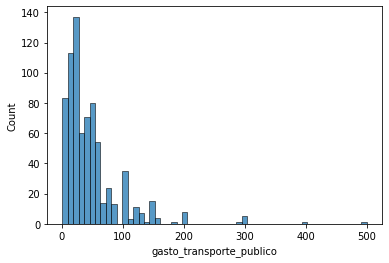
\includegraphics[width = 0.9 \textwidth]{stcase01_gasto_tpublico_distri_presencia}
        \caption{Distribución del gasto, en zonas \textbf{con presencia de vandalismo}}
    \end{subfigure}
    \begin{subfigure}[b]{0.45 \textwidth}
        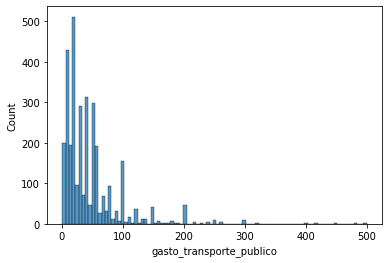
\includegraphics[width = 0.9 \textwidth]{stcase01_gasto_tpublico_distri_nopresencia}
        \caption{Distribución del gasto, en zonas \textbf{sin presencia de vandalismo}}
    \end{subfigure}


    \caption{Distribuciones de gasto en transporte público de las dos poblaciones estudiadas, según presencia o no de vandalismo en la zona del hogar}
\end{figure}


A raíz de estas dos distribuciones, apenas podemos sacar conclusiones adicionales a simple vista. Ambas distribuciones tienen una forma muy similar, que se diferencia tan solo en que en la población sin presencia de vandalismo supone un mayor número, y por tanto en la gráfica se muestran con mayor granularidad. El hecho de que ambas distribuciones sean prácticamente iguales en forma se ve claramente en las marcas en el eje de las $x$. Podemos ver los picos centrados en el gasto 200, 300, 400 y 500. Ademas, toda la distribución hasta que llegamos a gasto 100 es prácticamente idéntica (salvo la granularidad ya comentada).

Por esto, cobra mayor interés estudiar el efecto de usar el gasto en transporte para la clusterización, pues esto puede descubrir patrones que a simple vista no hemos sido capaces de captar.

Aprovechamos la sección de exploración de datos de este caso de estudio para realizar la siguiente observación, que tendrá impacto en el resto de casos de estudio. En un primer momento, consideramos usar las variables

\lstinline{renta_disponible_total_hogar}

y

\lstinline{renta_disponible_restado_alquiler}.

Sin embargo, como mostramos a continuación, están muy correladas, por lo que no aportan información interesante:

\begin{figure}[H]
    \centering

    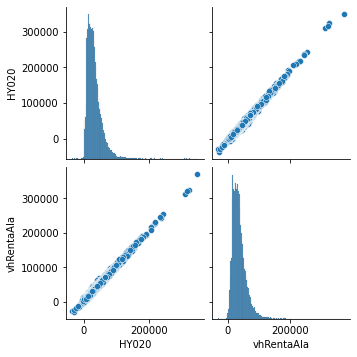
\includegraphics[width = 0.6 \textwidth]{stcase01_correlacion_renta_total_restado}
    \caption{Gráfico en el que se aprecia claramente la correlación entre la variable \lstinline{renta_disponible_total_hogar} y la variable \lstinline{renta_disponible_restado_alquiler}}
\end{figure}

Lo mismo ocurre con la variable agregada por nosotros, \lstinline{ingresos_menos_gastos}, y la variable ya presente en los datos originales, \lstinline{renta_disponible_total_hogar}. Esto se muestra claramente en la siguiente gráfica:

\begin{figure}[H]
    \centering

    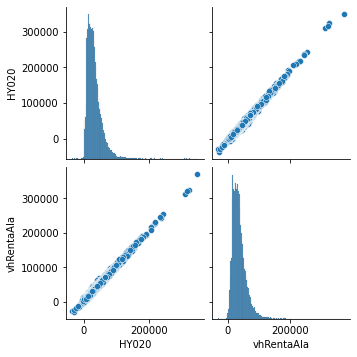
\includegraphics[width = 0.6 \textwidth]{stcase01_correlacion_renta_total_mi_variable_agregada}
    \caption{Gráfico en el que se aprecia claramente la correlación entre la variable \lstinline{renta_disponible_total_hogar} y la variable agregada \lstinline{renta_disponible_restado_alquiler}}
\end{figure}

Por tanto, no tiene sentido usar ambas variables en un mismo caso de estudio, pues apenas aportan información nueva al problema, debido a la alta correlación entre ambas.

\pagebreak

\subsection{Resultados de \emph{clustering}} \label{stcase01_parametros:seccion}

Aplicamos \emph{clustering} con los siguientes parámetros:

\begin{enumerate}
    \item \lstinline{K-means}: total de \emph{clusters} 4
    \item \lstinline{DBSCAN}: $\epsilon = 0.4$, mínimo de ejemplos 1
    \item \lstinline{BIRCH}: total de \emph{clusters} 4, \emph{threshold} 0.2
    \item \lstinline{Mean Shift}: banda de 0.2, 1000 iteraciones máximas
    \item \emph{Clustering} aglomerativo: total de \emph{cluters} 4, técnica \entrecomillado{ward}
\end{enumerate}

Antes de mostrar la tabla con las métricas de los algoritmos, mostramos gráficamente los resultados obtenidos:

\begin{figure}[H]
    \centering

    \begin{subfigure}[b]{0.45 \textwidth}
        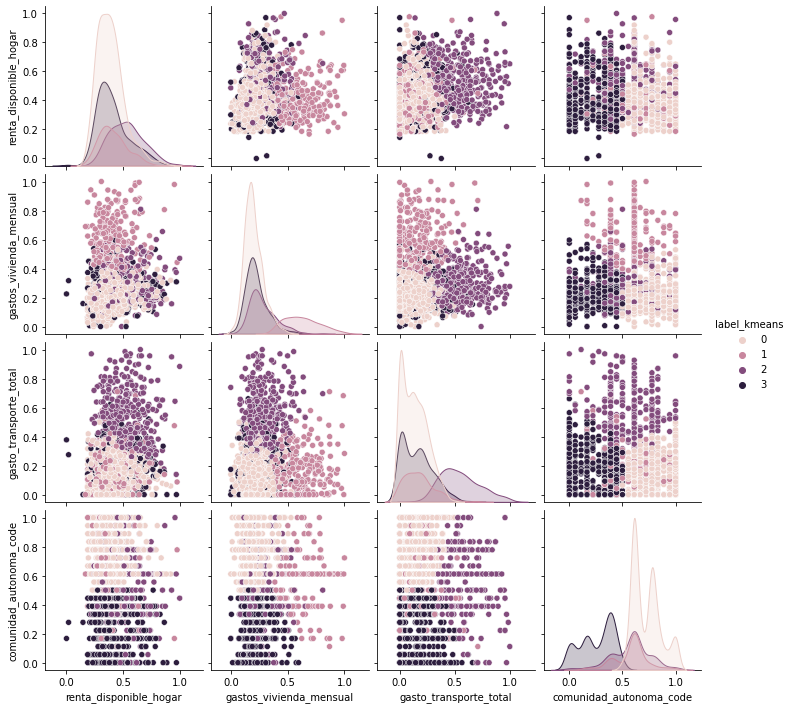
\includegraphics[width = 0.9 \textwidth]{stcase01_resultadografico_kmeans}
        \caption{\lstinline{K-Means}}
    \end{subfigure}
    \begin{subfigure}[b]{0.45 \textwidth}
        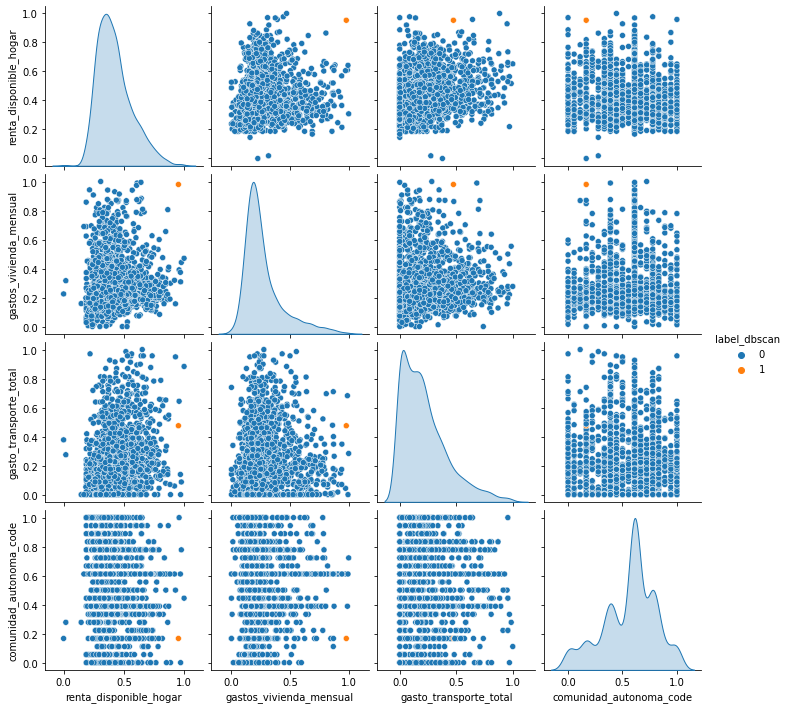
\includegraphics[width = 0.9 \textwidth]{stcase01_resultadografico_DBSCAN}
        \caption{\lstinline{DBSCAN}}
    \end{subfigure}

    \begin{subfigure}[b]{0.45 \textwidth}
        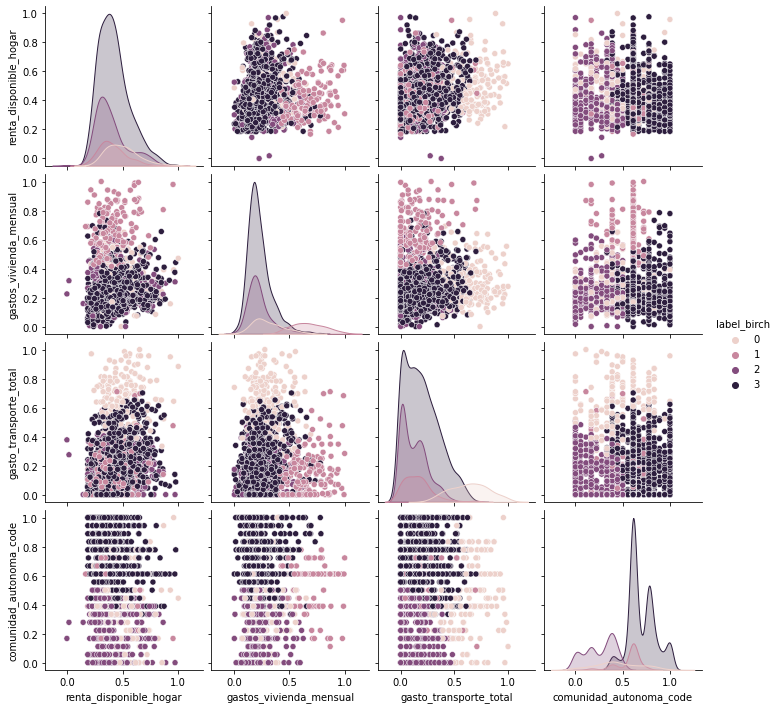
\includegraphics[width = 0.9 \textwidth]{stcase01_resultadografico_BIRCH}
        \caption{\lstinline{BIRCH}}
    \end{subfigure}
    \begin{subfigure}[b]{0.45 \textwidth}
        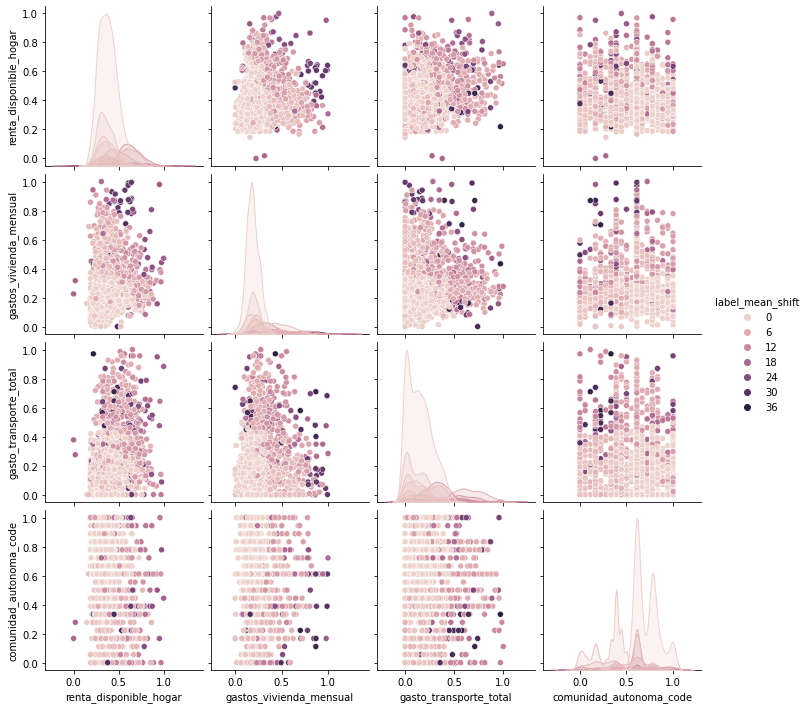
\includegraphics[width = 0.9 \textwidth]{stcase01_resultadografico_MEANSHIFT}
        \caption{\lstinline{Mean-Shift}}
    \end{subfigure}

    \begin{subfigure}[b]{0.45 \textwidth}
        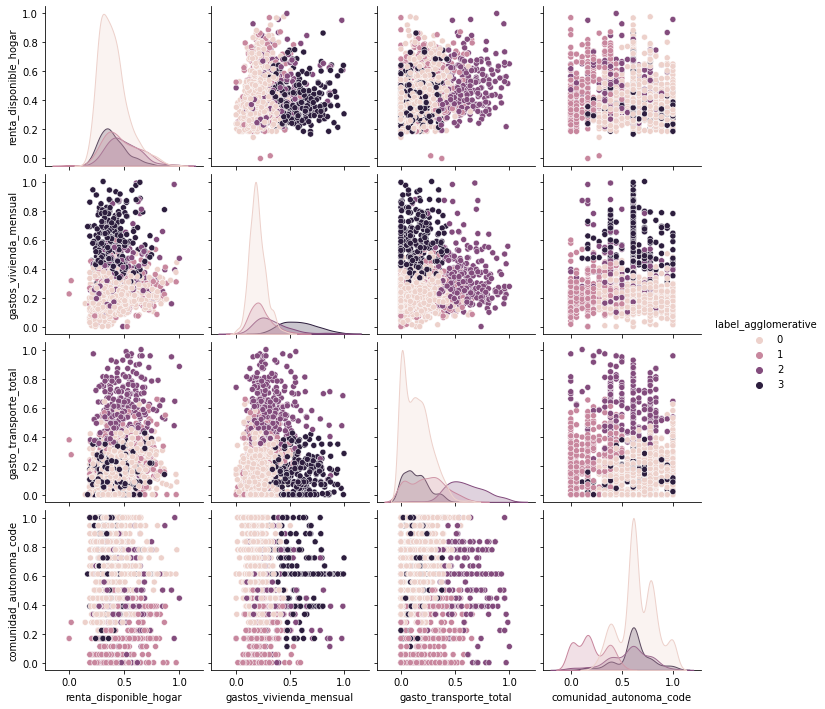
\includegraphics[width = 0.9 \textwidth]{stcase01_resultadografico_AGLOMERATIVO}
        \caption{\emph{Clustering} aglomerativo}
    \end{subfigure}


    \caption{Resultados gráficos tras aplicar los distintos algoritmos de \emph{clustering}. Realizamos la misma gráfica \emph{pairplot}, pero coloreando según el \emph{cluster} que hemos asignado}
    \label{stcase01_resultados_graficos:figure}

\end{figure}

Destacan los malos resultados obtenidos a simple vista por \lstinline{DBSCAN}. Solo logra colocar un punto en un \emph{cluster}, dejando el resto del dataset al otro \emph{cluster} generado. Como veremos más adelante, esta es una forma de lograr un valor de \emph{Silhouette} muy bueno. Por tanto, este ejemplo sirve para motivar el resto de métricas que hemos empleado para evaluar los \emph{cluters}.

El resto de algoritmos parece tener resultados bastantes buenos. Quizás destaca algo \emph{Mean Shift}, pues genera demasiados \emph{clusters} para el problema que estamos tratando (concretamente, genera 36 \emph{clusters}). Así que tendremos que vigilar ciertas métricas respecto a este algoritmo, para ver si obtiene buenos resultados según los criterios que hemos introducido.

El resto de \emph{clusters} parecen muy buenos, teniendo resultados bastante parecidos. Fijémonos por ejemplo en los resultados de \emph{BIRCH}. Empezando por las distribuciones de las variables, podemos fijarnos en que ha tomado un \emph{cluster} (el \emph{cluster} con etiqueta 3) con una renta media, un gasto moderado (tanto en hogar como en transporte) y que tiene mucha concentración en ciertas comunidades. De hecho, es el \emph{cluster} que más se concentra por comunidad autónoma. Sería interesante saber cuál es esa comunidad autónoma, pero por cuestiones de tiempo nos conformamos con la información que hemos expuesto. Podemos pensar que esto se debe a que es el \emph{cluster} con mayor número de elementos. Siguiendo en menor medida las tendencias del \emph{cluster} 3, tenemos el \emph{cluster} 2, con la segunda mayor renta y gasto.

El \emph{cluster} 3 es el que más bajo está en el ratio gastos en vivienda / renta disponible, mientras que el \emph{cluster} 1 es el más alto. El \emph{cluster} 0 es el que más gasta en transporte y en vivienda, en relación a la renta total. Por tanto, podemos pensar que el algoritmo de \emph{clusterización} ha encontrado un perfil de persona que gasta mucho en relación a lo que gana.

Con estas visualizaciones y estas apreciaciones sobre los perfiles encontrados, pasamos a mostrar las métricas obtenidas por los algoritmos:

\begin{table}[H]
\begin{center}
    \resizebox{1.05\textwidth}{!}{
    \begin{tabular}{|c|c|c|c|c|c|c|c|c|}
        \hline
        nombre & calinski & davies & elements mean & elements std & time & silhouette & total clusters & unbalanced \\

        \hline
        kmeans &  735.23 &  1.08 &  486.75 &  240.54 &  0.21 &  0.31 &  4 & 0.92 \\
        dbscan &  6.78 &  0.35 &  973.50 &  972.50 &  2.23 &  0.51 &  2 & 0.01 \\
        birch &  550.25 &  1.13 &  486.75 &  399.34 &  0.21 &  0.28 &  4 & 0.78 \\
        mean shift &  131.13 &  1.08 &  52.62 &  139.62 &  17.18 &  0.17 &  37 & 0.60 \\
        agglomerative &  552.65 &  1.22 &  486.75 &  359.85 &  0.19 &  0.26 &  4 & 0.83 \\
    \hline
    \end{tabular}}
\end{center}
\caption{Resultados de los algoritmos según distintas métricas de evaluación}
    \label{resultados_stcase01:tabla}
\end{table}

Lo primero que debemos explicar es qué significan ciertas métricas. \emph{elements mean} y \emph{elements std} son la media y desviación típica del número de elementos por \emph{cluster}. \emph{Unbalanced} es una métrica que hemos introducido para mirar el balanceo de la asignación de objetos a \emph{clusters}. Para ello, nos hemos inspirado en la siguiente contestación en un foro \emph{online} \cite{entropy_for_unbalanced:online}.

La idea es bastante básica. Partimos de la conocida entropía, que se usa normalmente para medir la incertidumbre de cierta información:

$$H = - \sum p_i \cdot log_2(p_i)$$

La entropía se hace 0 cuando tenemos solo una clase con todos los datos, es decir, cuando el desbalanceo es el más alto (peor caso). No hay incertidumbre en la información. La entropía se hace máximo cundo el balanceo es perfecto, es decir, cuando distribuimos $n$ elementos en $k$ clases con $\frac{n}{k}$ elementos por cada clase. En cuyo caso, el valor máximo es $H = log(k)$. Para hacer que nuestra métrica esté en el rango $[0, 1]$, normalizamos tal que:

$$unbalanced = \frac{H}{log(k)}$$

Con esto, buscamos que esta métrica tome valores lo más cercanos a 1, para que la distribución en \emph{clusters} no sea un caso extremo (por ejemplo, como ya hemos visto, un punto en un \emph{cluster} y el resto en otro \emph{cluster}).

Antes de interpretar los resultados de la tabla \customcite{resultados_stcase01:tabla}, mostramos las métricas de forma gráfica, pues esto facilitará la comprensión de dichas métricas y el comportamiento de los algoritmos. Decidimos no mostrar las dos gráficas asociadas a las métricas de los elementos, pues es una información que estamos resumiendo en la métrica \emph{unbalanced}.

\begin{figure}[H]
    \centering

    \begin{subfigure}[b]{0.45 \textwidth}
        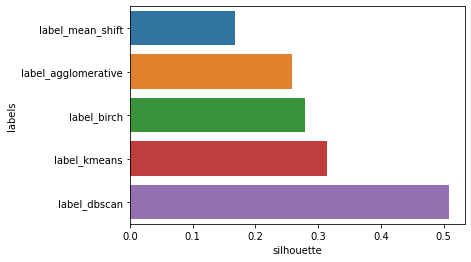
\includegraphics[width = 0.9 \textwidth]{stcase01_metricagrafica_silhouette}
        \caption{Silhouette}
    \end{subfigure}
    \begin{subfigure}[b]{0.45 \textwidth}
        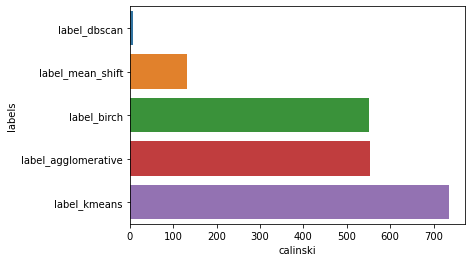
\includegraphics[width = 0.9 \textwidth]{stcase01_metricagrafica_calinski}
        \caption{Calinski}
    \end{subfigure}

    \begin{subfigure}[b]{0.45 \textwidth}
        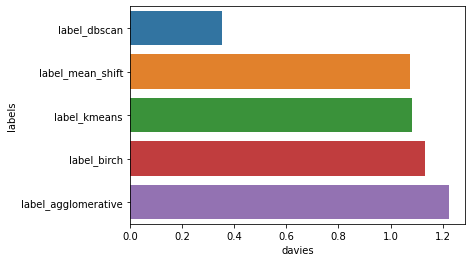
\includegraphics[width = 0.9 \textwidth]{stcase01_metricagrafica_davies}
        \caption{Davies}
    \end{subfigure}
    \begin{subfigure}[b]{0.45 \textwidth}
        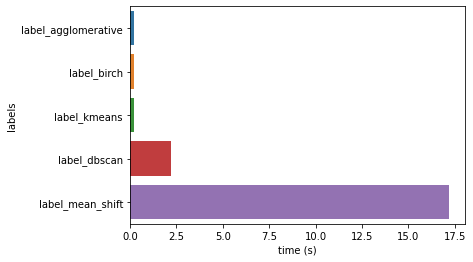
\includegraphics[width = 0.9 \textwidth]{stcase01_metricagrafica_time}
        \caption{Tiempo de ejecución}
    \end{subfigure}

    \begin{subfigure}[b]{0.45 \textwidth}
        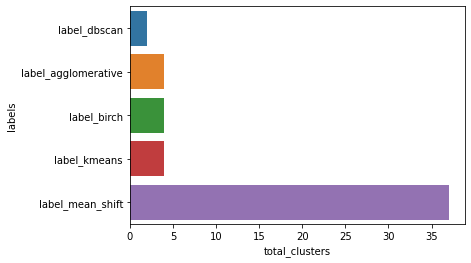
\includegraphics[width = 0.9 \textwidth]{stcase01_metricagrafica_total_clusters}
        \caption{Número total de clusters}
    \end{subfigure}
    \begin{subfigure}[b]{0.45 \textwidth}
        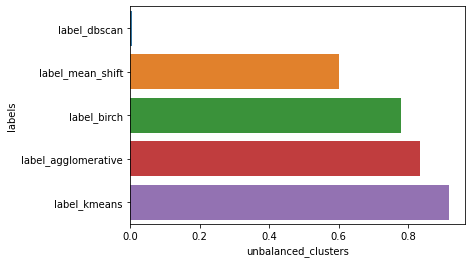
\includegraphics[width = 0.9 \textwidth]{stcase01_metricagrafica_total_unbalanced}
        \caption{Métrica \emph{unbalanced}}
    \end{subfigure}

    \caption{Gráficas con las distintas métricas que hemos construido}
    \label{stcase01_metricas_graficas:figure}
\end{figure}

Con toda esta información, podemos proceder a realizar ciertas conclusiones sobre los algoritmos de \emph{clusterización}.

\pagebreak

\subsection{Interpretación de los resultados de \emph{clustering}}

Lo que más resalta es que en \customcite{stcase01_metricas_graficas:figure} veamos que, fijándonos en \emph{Silhouette}, el mejor algoritmo sea \emph{DBSCAN}, pero que en \customcite{stcase01_resultados_graficos:figure} sea claro que hemos obtenido un resultado desastroso, realizando lo que podría considerarse un \emph{clustering} trivial: un punto en un \emph{cluster} y el resto de puntos en otro \emph{cluster}. Esto es un problema conocido de la métrica \emph{Silhouette}, puede tomar buenos resultados si consigue hacer esto mismo con un punto alejado lo suficientemente del resto (ie. con un outlier). Si nos fijamos en otras métricas, como Calinski o Davies, vemos que \emph{DBSCAN} es el algoritmo con peores resultados. Pero si nos fijamos en nuestra métrica \emph{unbalanced}, es claro lo desastroso del resultado, al ser evidente que tenemos una asignación muy desbalanceada, cercana al peor caso en el que la métrica es cero. Por tanto, estamos viendo con un ejemplo que la métrica Silhouette no es suficiente por sí sola para evaluar la calidad de un algoritmo de clusterización.

Fijándonos en las otras métricas, podemos concluir que los mejores algoritmos son \emph{K-Means}, \emph{Clusterización Aglomerativa} y \emph{BIRCH}. \emph{Mean Shift} no obtiene buenos resultados. Genera un número demasiado elevado de clusters, teniendo una mala métrica de \emph{unbalanced} sin llegar a ser catastrófica. Además, es el algoritmo que más tarda en ejecutarse, sobresaliendo respecto al resto de algoritmos significativamente.

\emph{K-means} obtiene resultados sorprendentemente competitivos, teniendo en cuenta la simplicidad de este algoritmo. Es el algoritmo que mejor balancea la asignación a \emph{clusters}, como era de esperar por la propia naturaleza del algoritmo.

El segundo mejor algoritmo en balanceo es el aglomerativo. La naturaleza de dicho algoritmo también nos hacía sospechar de los buenos resultados respecto de esta métrica. Sin embargo, lo que sí sorprende son los buenos resultados en las otras métricas. Estamos obteniendo resultados muy competitivos con el añadido de disponer una jerarquía que nos da más información sobre el problema.

\pagebreak

\subsection{Visualizando en 2D las clusterizaciones}

Usaremos dos técnicas, \lstinline{PCA} y \lstinline{TSNE}, para realizar visualizaciones de la \emph{clusterización} en dos dimensiones. A continuación mostramos los resultados de \emph{PCA}:

\begin{figure}[H]
    \centering

    \begin{subfigure}[b]{0.45 \textwidth}
        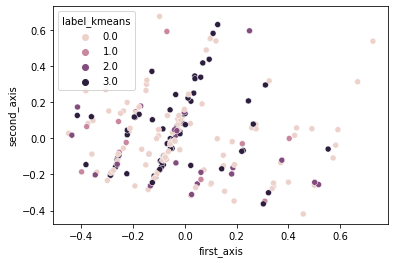
\includegraphics[width = 0.9 \textwidth]{stcase01_pca_kmeans}
        \caption{K-Means}
    \end{subfigure}
    \begin{subfigure}[b]{0.45 \textwidth}
        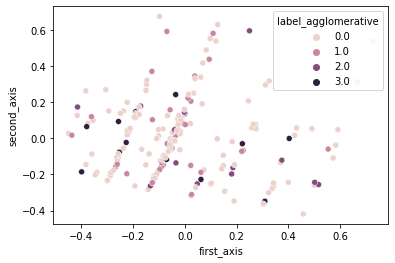
\includegraphics[width = 0.9 \textwidth]{stcase01_pca_aglomerativo}
        \caption{\emph{Clustering} aglomerativo}
    \end{subfigure}

    \begin{subfigure}[b]{0.45 \textwidth}
        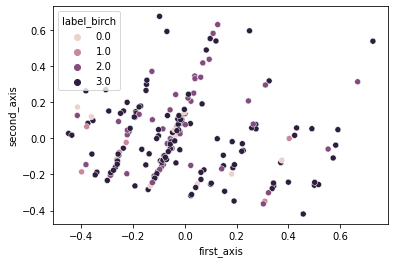
\includegraphics[width = 0.9 \textwidth]{stcase01_pca_birch}
        \caption{Birch}
    \end{subfigure}
    \begin{subfigure}[b]{0.45 \textwidth}
        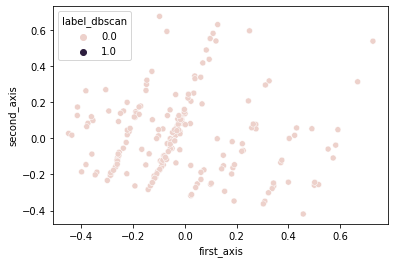
\includegraphics[width = 0.9 \textwidth]{stcase01_pca_dbscan}
        \caption{DBSCAN}
    \end{subfigure}

    \begin{subfigure}[b]{0.45 \textwidth}
        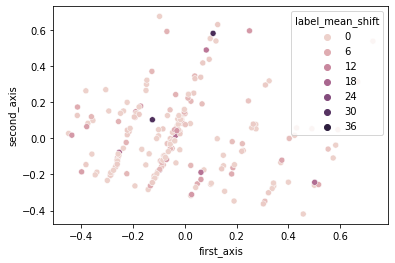
\includegraphics[width = 0.9 \textwidth]{stcase01_pca_meanshift}
        \caption{MeanShift}
    \end{subfigure}

        \caption{Resultados de las clusterizaciones, visualizadas en el espacio generado usando \emph{PCA}}
\end{figure}

Mostramos ahora los resultados aplicando \emph{tsne}. Esta técnica, aplicada explorando muchos valores de sus parámetros, nos puede dar cierta idea de la topología de los datos con los que se trabajan \cite{tsne:online}. Sin embargo, por falta de tiempo y para evitar una gran extensión en esta memoria, solo mostramos los resultados con unos parámetros fijos:

\begin{figure}[H]
    \centering

    \begin{subfigure}[b]{0.45 \textwidth}
        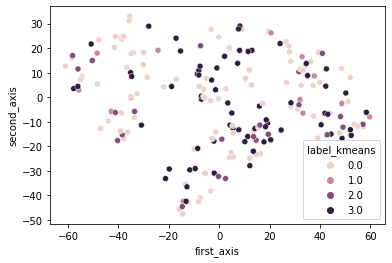
\includegraphics[width = 0.9 \textwidth]{stcase01_tsne_kmeans}
        \caption{K-Means}
    \end{subfigure}
    \begin{subfigure}[b]{0.45 \textwidth}
        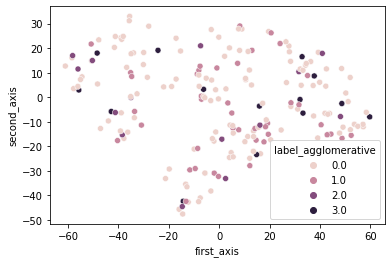
\includegraphics[width = 0.9 \textwidth]{stcase01_tsne_aglomerativo}
        \caption{\emph{Clustering} aglomerativo}
    \end{subfigure}

    \begin{subfigure}[b]{0.45 \textwidth}
        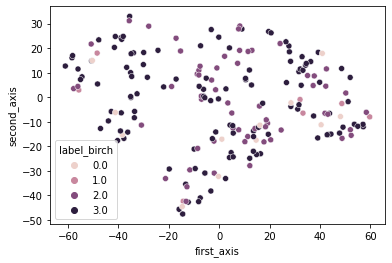
\includegraphics[width = 0.9 \textwidth]{stcase01_tsne_birch}
        \caption{Birch}
    \end{subfigure}
    \begin{subfigure}[b]{0.45 \textwidth}
        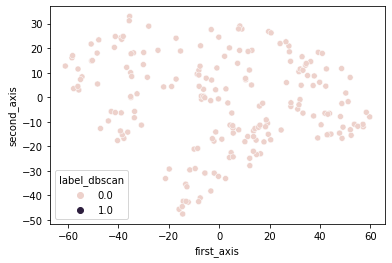
\includegraphics[width = 0.9 \textwidth]{stcase01_tsne_dbscan}
        \caption{DBSCAN}
    \end{subfigure}

    \begin{subfigure}[b]{0.45 \textwidth}
        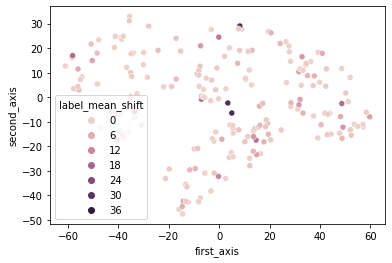
\includegraphics[width = 0.9 \textwidth]{stcase01_tsne_meanshift}
        \caption{MeanShift}
    \end{subfigure}

        \caption{Resultados de las clusterizaciones, visualizadas en el espacio generado usando \emph{tsne}}
\end{figure}

Con estas gráficas podemos sacar poca información adicional respecto a lo que ya hemos comentado previamente. Es claro que los resultados de \emph{DBSCAN} son completamente desastrosos. Visualmente, parece que \emph{K-means} y \emph{Clustering Aglomerativo} son los algoritmos que descubren relaciones más equilibradas y complejas. En el resto de algoritmos, hay cierta dominancia por parte de determinados \emph{clusters} (ie. el cluster 0 en \emph{mean shift}).

En último lugar, no parece que \emph{tsne} haya servido para descubrir ciertas propiedades topológicas del conjunto de datos con el que trabajamos, ni estamos viendo correlaciones entre agrupaciones gracias a \emph{tsne} y nuestros algoritmos de \emph{clusterización}. No podemos concluir nada con esto, pues como ya hemos comentado, no estamos explorando distintas combinaciones de parámetros para \emph{tsne}.

Hemos creado también una gráfica en la que mostramos los \emph{clusters} obtenidos de forma simplificada. Para ello, mostramos los centroides con el tamaño proporcional al radio del \emph{cluster} y con el color proporcional al número de elementos del \emph{cluster}. Estas dos métricas las calculamos nosotros, trabajando directamente con los \lstinline{dataframes}. En algunos algoritmos se puede obtener esta información accediendo a los atributos del clasificador, pero no en todos. Por tanto, decidimos calcular estas métricas manualmente, como acabamos de decir. Además, aplicamos \emph{tsne} para realizar esta visualización en dos dimensiones. Los resultados obtenidos son los siguientes:

\begin{figure}[H]
    \centering

    \begin{subfigure}[b]{0.45 \textwidth}
        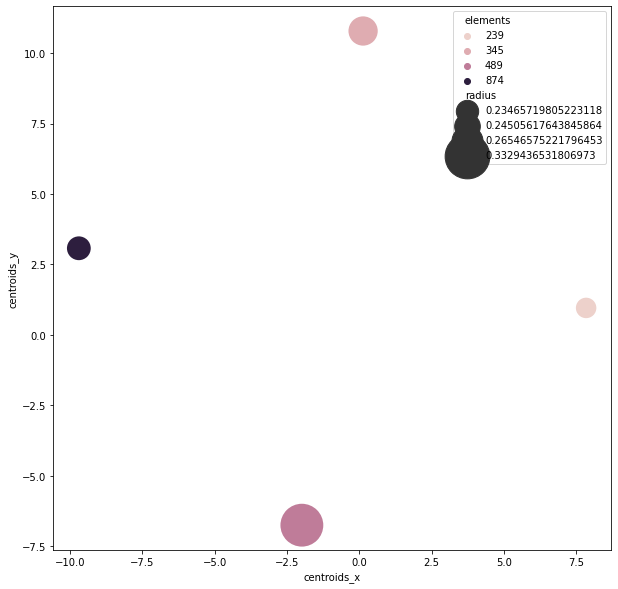
\includegraphics[width = 0.9 \textwidth]{stcase01_centroides_kmeans}
        \caption{K-Means}
    \end{subfigure}
    \begin{subfigure}[b]{0.45 \textwidth}
        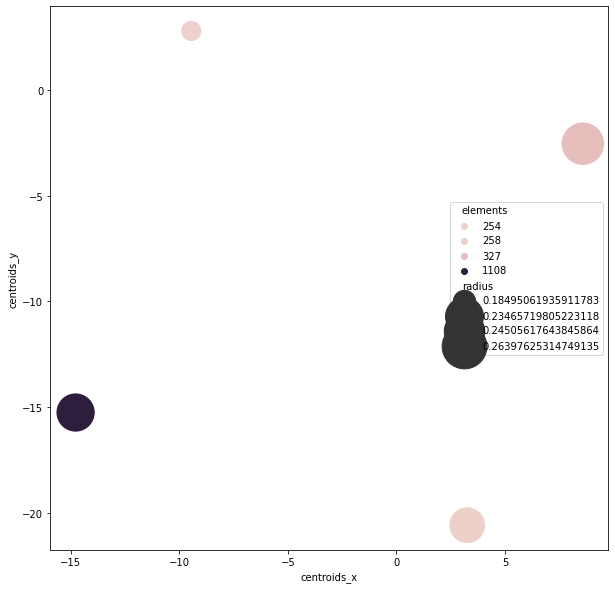
\includegraphics[width = 0.9 \textwidth]{stcase01_centroides_aglomerativo}
        \caption{\emph{Clustering} aglomerativo}
    \end{subfigure}

    \begin{subfigure}[b]{0.45 \textwidth}
        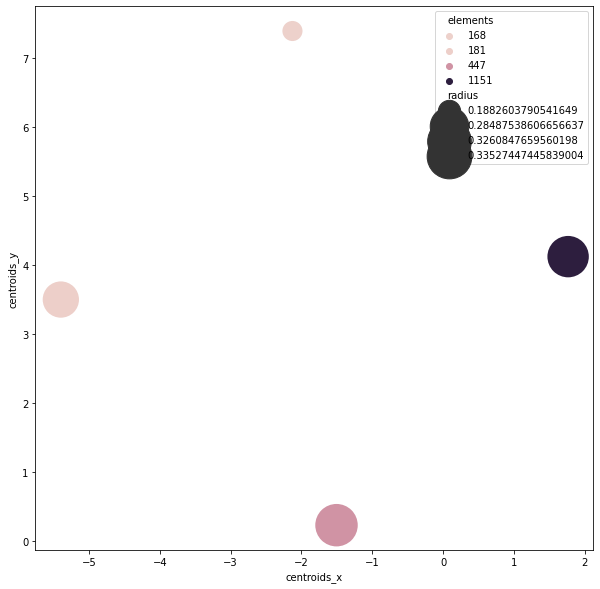
\includegraphics[width = 0.9 \textwidth]{stcase01_centroides_birch}
        \caption{Birch}
    \end{subfigure}

        \caption{Gráfica que hemos descrito previamente, para los distintos algoritmos de \emph{clusterización usados en la práctica}}
\end{figure}

Notar que no se incluyen las gráficas ni de \emph{DBSCAN} ni de \emph{Mean Shift}. Esto porque la clusterización realizada provoca que no podamos computar ciertas métricas (en ambos, tenemos \emph{clusters} con solo un punto).

En los tres algoritmos que podemos visualizar, vemos que hemos acabado con cuatro \emph{clusters} que forman aproximadamente un rombo, con centroides muy parecidos en posición. Aquí también se visualiza que \emph{K-Means} es el algoritmo que mejor distribuye los elementos por \emph{cluster}. Aunque no vamos a entrar en estudiar esto, porque para ello ya hemos discutido nuestra métrica \emph{unbalanced}. Por tanto, parece que salvo pequeñas diferencias, los cuatro algoritmos generan \emph{clusters} aparentemente muy parecidos.

Mostramos las coordenadas paralelas, coloreando con la \emph{clusterización} de cada algoritmo:

\begin{figure}[H]
    \centering

    \begin{subfigure}[b]{0.45 \textwidth}
        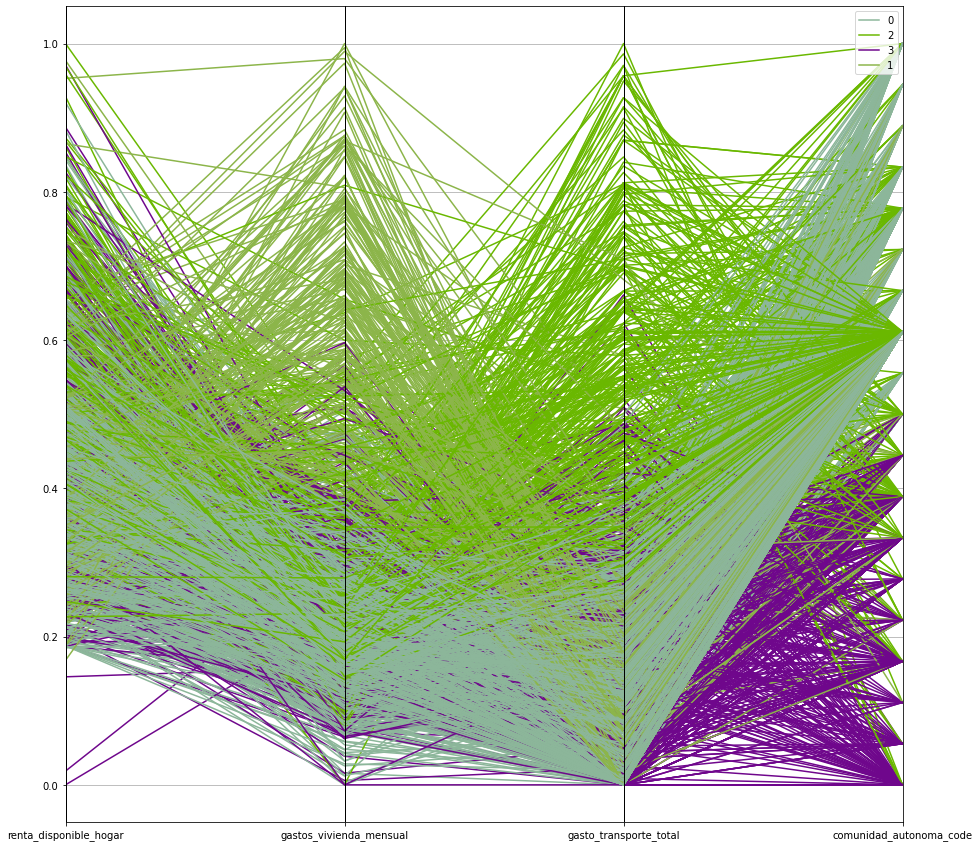
\includegraphics[width = 0.9 \textwidth]{stcase01_parallel_coordinates_kmeans}
        \caption{K-Means}
    \end{subfigure}
    \begin{subfigure}[b]{0.45 \textwidth}
        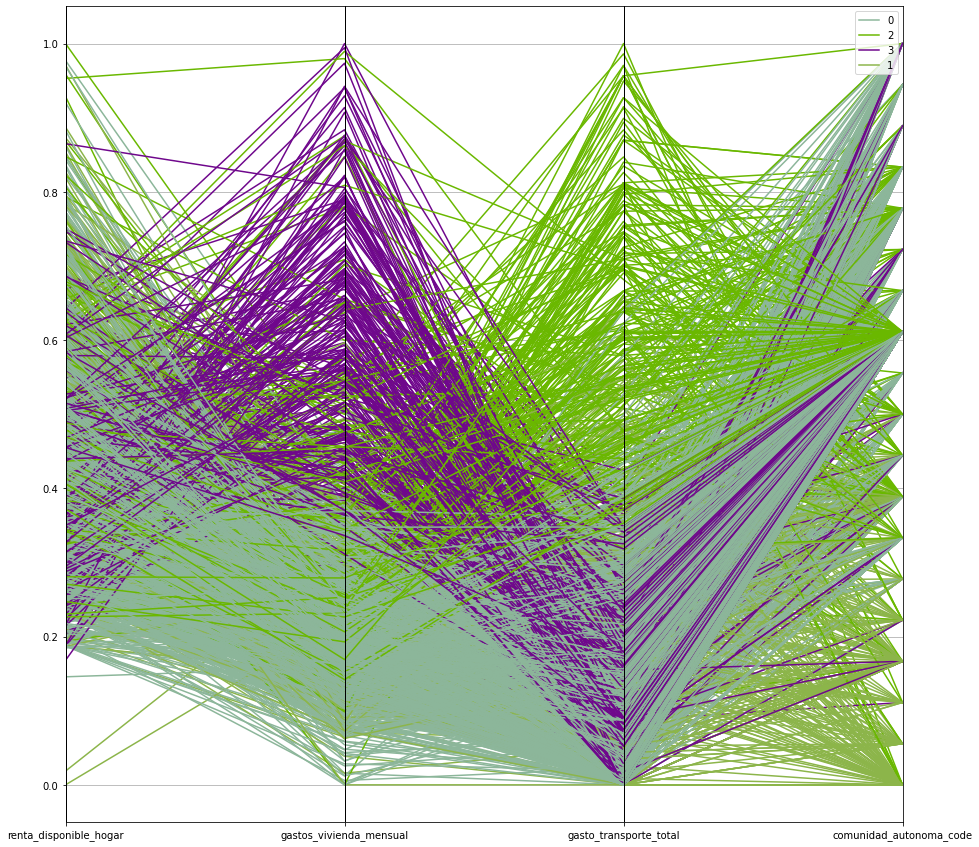
\includegraphics[width = 0.9 \textwidth]{stcase01_parallel_coordinates_aglomerativo}
        \caption{\emph{Clustering} aglomerativo}
    \end{subfigure}

    \begin{subfigure}[b]{0.45 \textwidth}
        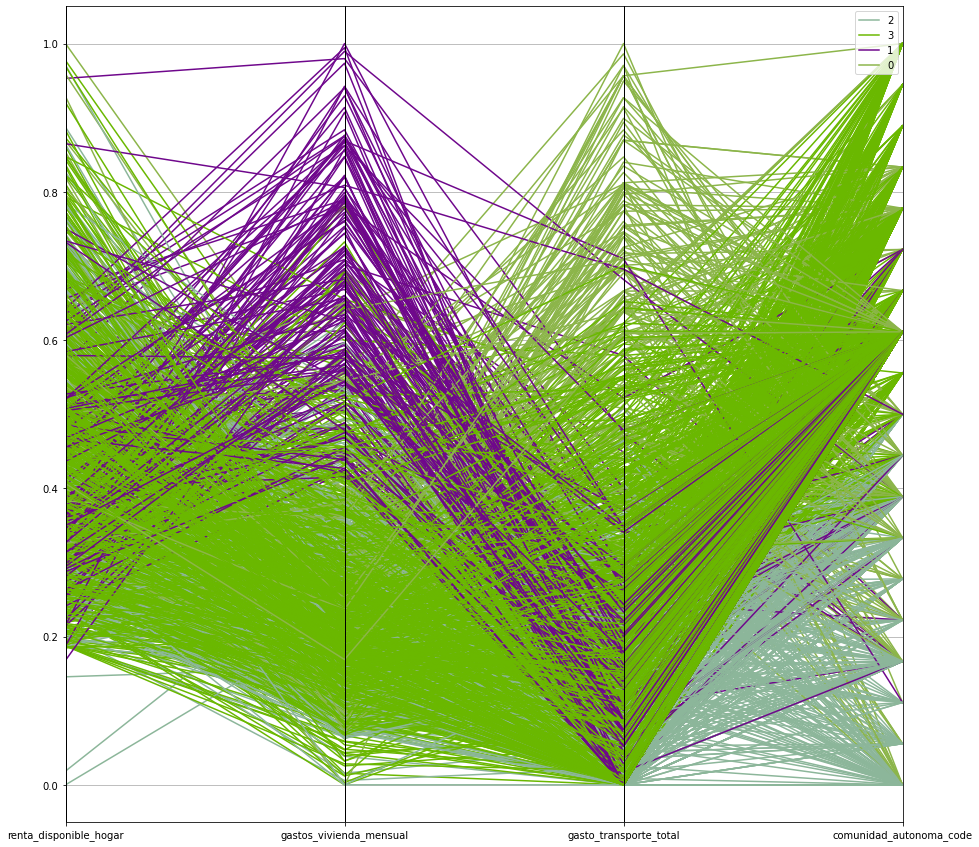
\includegraphics[width = 0.9 \textwidth]{stcase01_parallel_coordinates_birch}
        \caption{Birch}
    \end{subfigure}
    \begin{subfigure}[b]{0.45 \textwidth}
        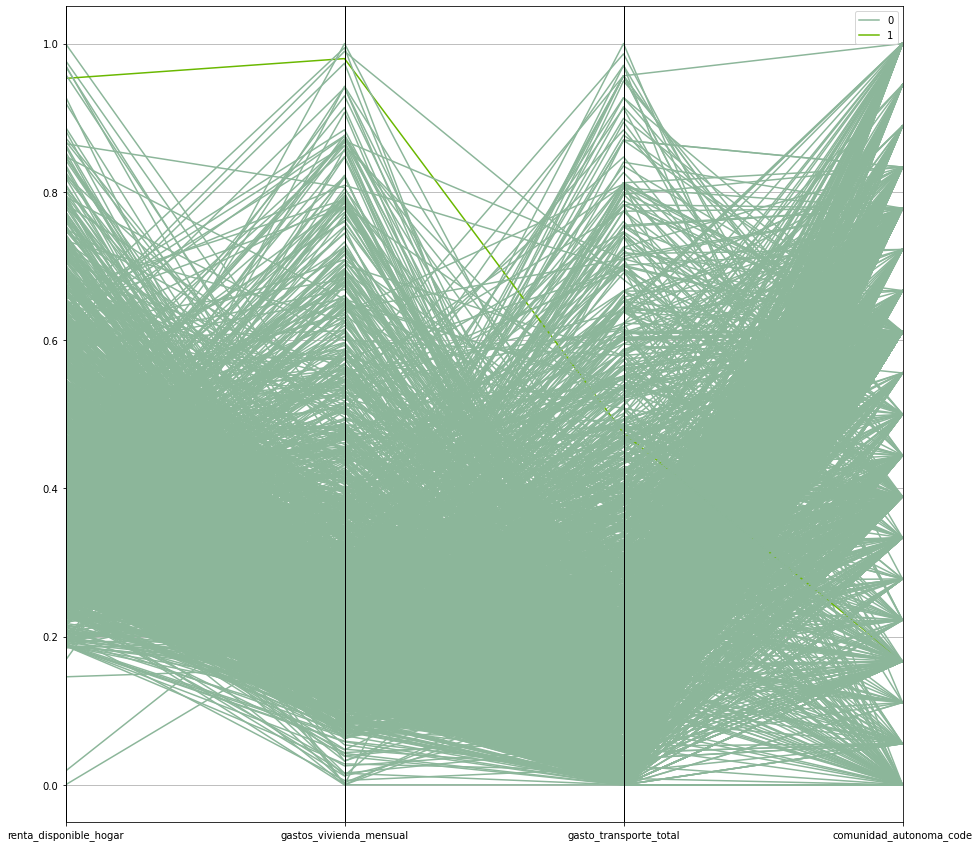
\includegraphics[width = 0.9 \textwidth]{stcase01_parallel_coordinates_dbscan}
        \caption{DBSCAN}
    \end{subfigure}

    \begin{subfigure}[b]{0.45 \textwidth}
        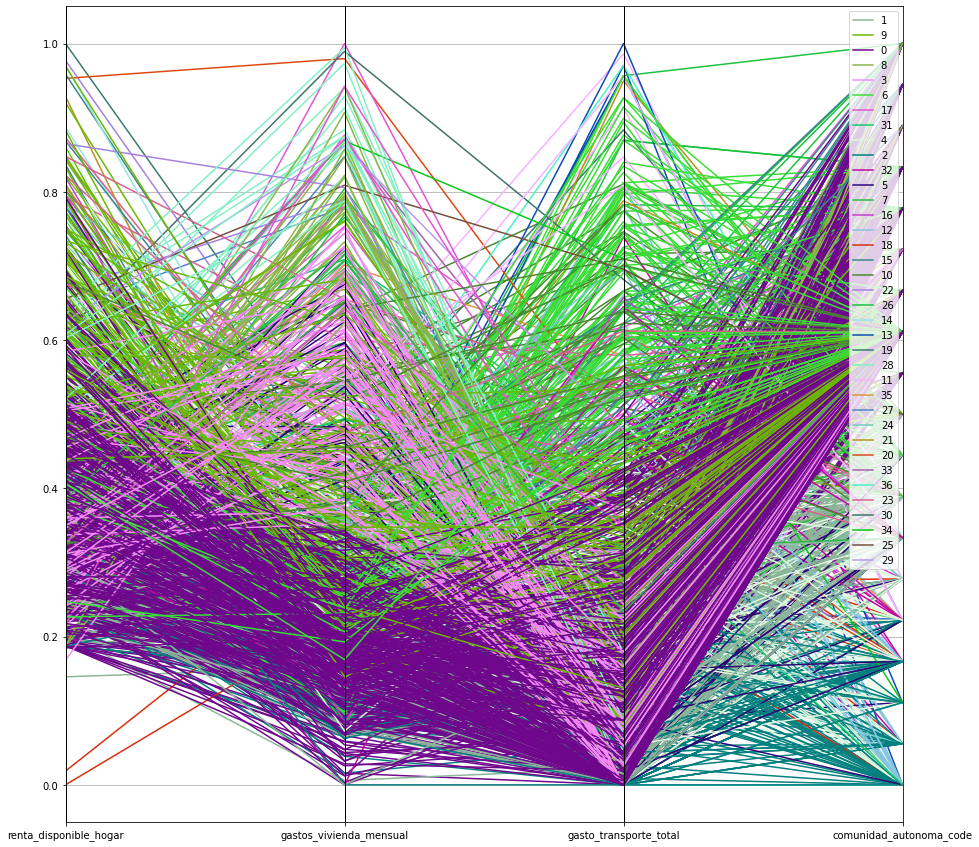
\includegraphics[width = 0.9 \textwidth]{stcase01_parallel_coordinates_meanshift}
        \caption{MeanShift}
    \end{subfigure}

    \caption{Gráfica coordenadas paralelas, coloreando con los distintos algoritmos de \emph{clusterización}}
\end{figure}

Los resultados desastrosos de \emph{DBSCAN} se hacen evidentes de nuevo. El resto de algoritmos, salvo \emph{Mean Shift}, muestran una complejidad similar, aunque los patrones descubiertos sean algo distintos. Sin embargo, \emph{Mean Shift} muestra unos patrones demasiado complejos para el problema que estamos resolviendo, como ya hemos comentado previamente.

Finalizamos este apartado mostrando los dendogramas obtenidos para cada algoritmo de \emph{clusterización}:

\begin{figure}[H]
    \centering

    \begin{subfigure}[b]{0.45 \textwidth}
        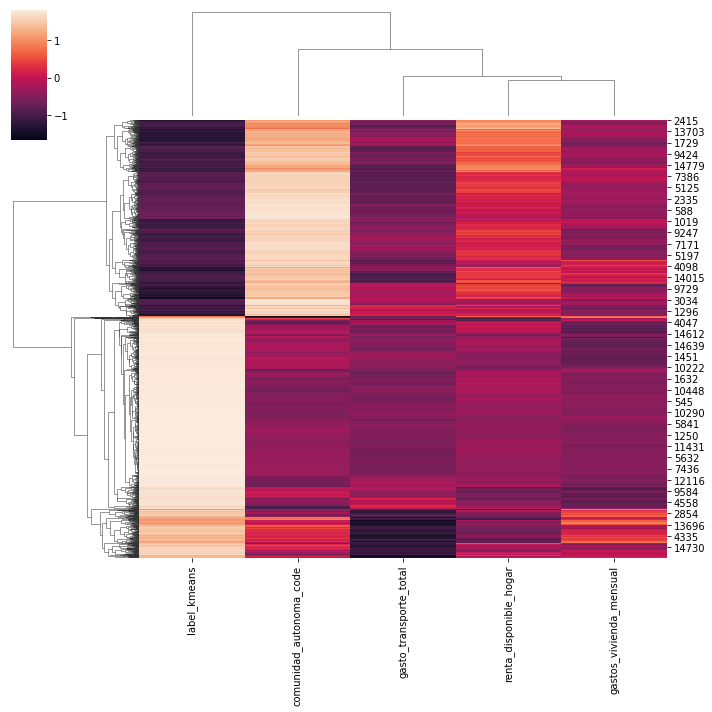
\includegraphics[width = 0.9 \textwidth]{stcase01_dendogram_kmeans}
        \caption{K-Means}
    \end{subfigure}
    \begin{subfigure}[b]{0.45 \textwidth}
        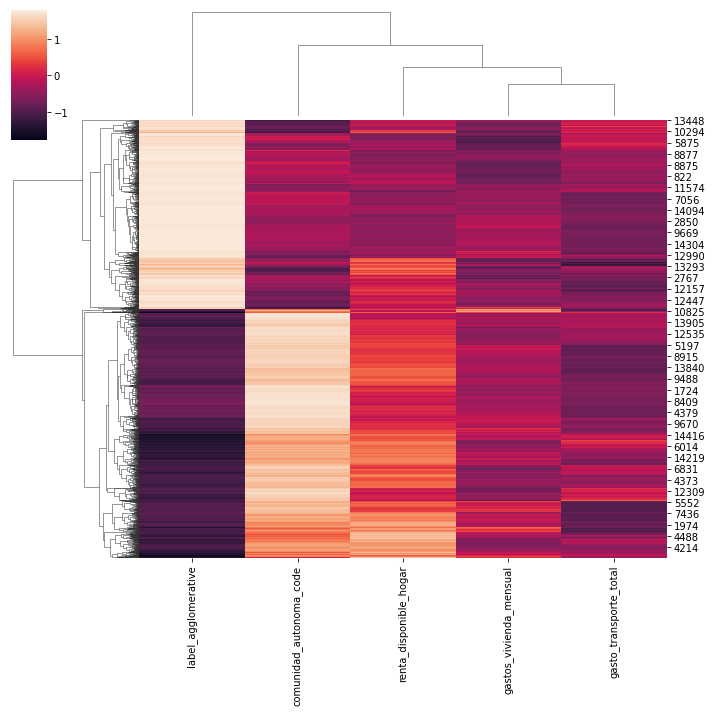
\includegraphics[width = 0.9 \textwidth]{stcase01_dendogram_aglomerativo}
        \caption{\emph{Clustering} aglomerativo}
    \end{subfigure}

    \begin{subfigure}[b]{0.45 \textwidth}
        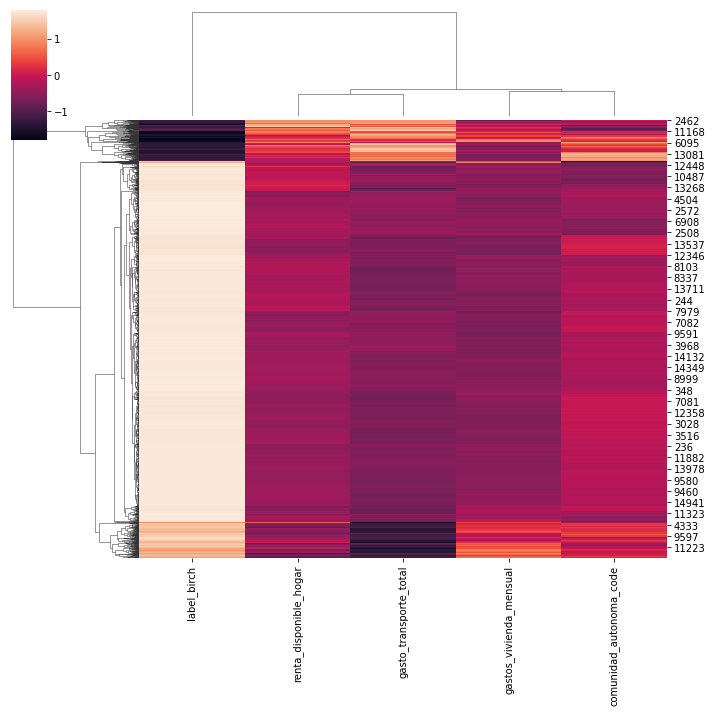
\includegraphics[width = 0.9 \textwidth]{stcase01_dendogram_birch}
        \caption{Birch}
    \end{subfigure}
    \begin{subfigure}[b]{0.45 \textwidth}
        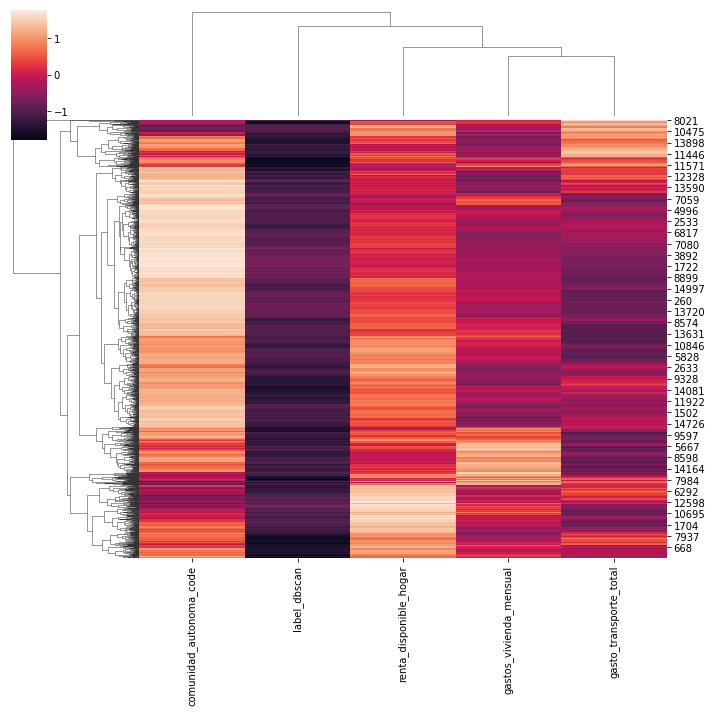
\includegraphics[width = 0.9 \textwidth]{stcase01_dendogram_dbscan}
        \caption{DBSCAN}
    \end{subfigure}

    \begin{subfigure}[b]{0.45 \textwidth}
        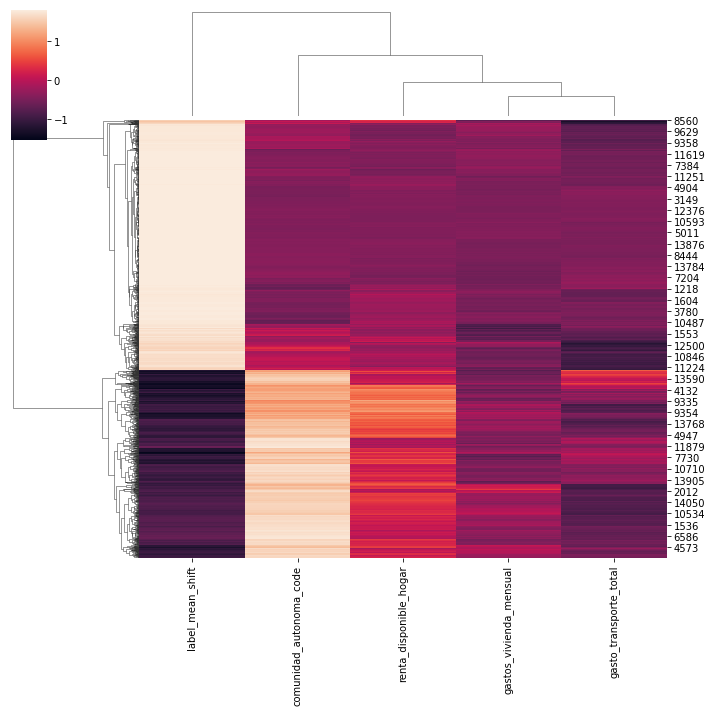
\includegraphics[width = 0.9 \textwidth]{stcase01_dendogram_meanshift}
        \caption{MeanShift}
    \end{subfigure}

    \caption{Dendograma de los distintos algoritmos de \emph{clusterización}}
\end{figure}

Se ve a simple vista que \emph{DBSCAN} es demasiado ruidoso, siendo difícil interpretar dicha gráfica. El resto de algoritmos, a simple vista, parecen tener comportamientos similares, incluso \emph{Mean Shift}.

\pagebreak

\subsection{Ajuste de los parámetros de los algoritmos}

En esta sección, decidimos ajustar los parámetros de \emph{K-Means} y de \emph{DBSCAN}. En un primer momento escogemos ajustar \emph{DBSCAN}, obteniendo los parámetros que hemos usado en \customcite{stcase01_parametros:seccion}. Como ya hemos visto, esto provoca obtener unos resultados nefastos. Decidimos dejar estos resultados malos para ilustrar el proceso erróneo que hemos seguido y la necesidad de tener en cuenta métricas más allá de \emph{Silhouette}.

Empezamos ajustando los parámetros de \emph{K-Means}. Los resultados de la exploración sobre estos parámetros se muestra en la siguiente tabla:

\begin{table}[H]
\begin{center}
    \begin{tabular}{|c|c|c|c|}
        \hline
        Número clusters & Silhouette & Calinski & unbalanced \\
        \hline
        1 &  -1.00 &  0.00 &  0.00 \\
        2 &  0.28 &  714.96 &  0.93 \\
        3 &  0.29 &  716.87 &  0.94 \\
        \textbf{4} &  \textbf{0.31} &  \textbf{735.23} &  \textbf{0.92} \\
        5 &  0.26 &  680.97 &  0.95 \\
        6 &  0.24 &  629.66 &  0.95 \\
        7 &  0.25 &  621.86 &  0.95 \\
        8 &  0.22 &  597.89 &  0.99 \\
        9 &  0.22 &  560.15 &  0.97 \\
        10 &  0.23 &  549.51 &  0.97 \\
        \hline
    \end{tabular}
\end{center}
    \caption{Resultados del ajuste de los parámetros de \emph{K-Means}}
    \label{resultados_stcase01:tabla}
\end{table}

Fijándonos en el índice de \emph{Silhouette}, nos quedamos con el parámetro 4 \emph{clusters} totales. Además, en la misma tabla podemos ver que esto genera \emph{clusters} bien balanceados.

Notar que en el código tenemos gráficas para mostrar la evolución de las distintas métricas en base al parámetro. Esto ha sido útil a la hora de explorar los rangos de los parámetros, pero la información es tan sencilla que no tiene sentido que mostremos aquí estos gráficos. Cuando ajustemos los parámetros de \emph{DBSCAN}, mostraremos gráficamente la evolución, pues la información obtenida es algo más compleja.

También es destacable el uso que hacemos de esta información. En todos los algoritmos en los que ha sido necesario fijar el número total de \emph{clusters}, hemos usado este valor. Por tanto, estamos usando esta exploración de parámetros y el algoritmo \emph{K-Means} como un método \emph{data-driven} para fijar los parámetros de otros algoritmos.

Mostramos ahora el ajuste realizado para los parámetros de \emph{DBSCAN}. Como se puede ver en el \emph{Notebook}, muchos de estos parámetros provocan obtener un \emph{Silhouette} nulo (al provocar el caso trivial de un único \emph{cluster}). Por simplicidad y claridad, en la siguiente tabla solo mostramos los valores de los parámetros que no provocan esta situación:


\begin{table}[H]
\begin{center}
    \begin{tabular}{|c|c|c|c|c|}
        \hline
            $\epsilon$ & Mín ejemplos & Silhouette & Calinski & unbalanced \\
        \hline

            0.30 & 1 &  0.44 &  6.20 &  0.01 \\
            0.30 & 2 &  0.44 &  6.20 &  0.01 \\
            0.30 & 3 &  0.44 &  6.20 &  0.01 \\
            0.30 & 4 &  0.44 &  6.20 &  0.01 \\
            0.30 & 5 &  0.44 &  6.20 &  0.01 \\
            0.30 & 6 &  0.44 &  6.20 &  0.01 \\
            \textbf{0.40} & \textbf{1} &  \textbf{0.51} &  \textbf{6.78} &  \textbf{0.01} \\
            0.40 & 2 &  0.51 &  6.78 &  0.01 \\
            0.40 & 3 &  0.51 &  6.78 &  0.01 \\
            0.40 & 4 &  0.51 &  6.78 &  0.01 \\
            0.40 & 5 &  0.51 &  6.78 &  0.01 \\
            0.40 & 6 &  0.51 &  6.78 &  0.01 \\

        \hline
    \end{tabular}
\end{center}
    \caption{Resultados del ajuste de los parámetros de \emph{DBSCAN}}
    \label{resultados_stcase01:tabla}
\end{table}

Claramente vemos que, con ninguno de los parámetros explorados que no provoca resultados triviales, conseguimos realizar una asignación balanceada. Así que lo único que importa en la selección de estos parámetros es el punto que dejamos aislado. Cuanto más alejado esté este punto del resto de puntos, mejores métricas obtendremos.

Como ya hemos comentado, mostramos gráficamente los resultados de la anterior tabla:

\begin{figure}[H]
    \centering

    \begin{subfigure}[b]{0.45 \textwidth}
        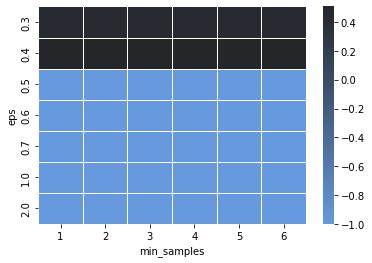
\includegraphics[width = 0.9 \textwidth]{stcase01_dbscan_explore_silh}
        \caption{Valor de \emph{Silhouette}}
    \end{subfigure}
    \begin{subfigure}[b]{0.45 \textwidth}
        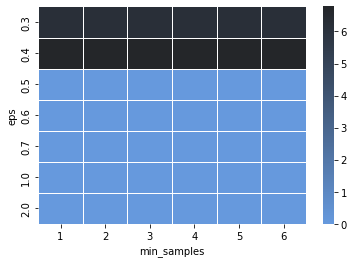
\includegraphics[width = 0.9 \textwidth]{stcase01_dbscan_explore_cal}
        \caption{Valor de \emph{Calinski}}
    \end{subfigure}

    \caption{\emph{Heatmap} de dos métricas relevantes, variando el valor de $\epsilon$ y el número mínimo de ejemplos}
\end{figure}

En ambas figuras, un valor más oscuro significa un mejor valor de la métrica. Más interesante que un análisis sobre lo que muestra la gráfica (los valores de $\epsilon$ son los que realmente marcan las métricas, siendo \lstinline{min_samples} irrelevante en este caso concreto), es más interesante destacar lo siguiente. Tanto la métrica \emph{Silhouette} como \emph{Calinski} muestran el mismo patrón. Y por tanto, parecen en parte insuficientes para ser capaces de capturar efectos como los que hemos descrito gracias a la métrica \emph{unbalanced} (\emph{clusterizaciones} triviales).

Con esto, podemos concluir que los resultados de \emph{dbscan} son desastrosos, y la exploración de parámetros no ha sido suficiente para encontrar un buen resultado. Creemos que esto podría solventarse con alguna de las siguientes alternativas:

\begin{enumerate}
    \item Realizar un borrado de \emph{outliers} más intenso, para evitar que \emph{DBSCAN} encuentre esos puntos aislados sobre los que colocar un \emph{cluster}. Sin embargo, a vista de la distribución de datos con la que trabajamos, esto no parece razonable, pues no tenemos una distribución con muchos puntos aislados
    \item Incluir, en la funcionalidad que computa el algoritmo, condiciones para evitar crear esos \emph{clusters} con un único punto aislado. Esto parece lo más adecuado por la flexibilidad y control que aporta, pero supondría re-escribir la funcionalidad de \lstinline{sklearn} o implementar nuestro propio algoritmo de \emph{clusterización} con estas opciones
\end{enumerate}


\pagebreak

\subsection{Interpretación de la segmentación}

% TODO -- poco gasto en transporte, como muestra \ref{stcase01_pairplot:figura}

\pagebreak

\section{Caso de estudio 2}

\pagebreak

\section{Caso de estudio 3}

\pagebreak

% Bibliografia
\bibliography{./References}
\bibliographystyle{ieeetr}

\end{document}
